\chapter{Modulación DSB-SC}
\label{sec.ej3:dsbsc}

La modulación en doble banda lateral con portadora suprimida se obtiene a partir del producto analógico directo
entre la señal modulante en banda base $e_m(t)$ y la señal portadora de radiofrecuencia $e_c(t)$. Considerando
tonos cosenoidales puros:
\begin{equation*}
    e_m(t) = E_m \cos(\omega_m t) \quad e_c(t) = E_c \cos(\omega_c t)
\end{equation*}
el producto resultante en la salida del modulador balanceado adopta la siguiente forma:
\begin{equation}
    v_{\mathrm{DSB}}(t) = e_m(t) \cdot e_c(t) = E_m E_c \cos(\omega_m t) \cos(\omega_c t)
    \label{eq.dsbsc:producto}
\end{equation}
Aplicando la identidad trigonométrica para el producto de cosenos, la expresión se descompone en dos frecuencias laterales:
\begin{equation}
    v_{\mathrm{DSB}}(t) = \frac{E_c E_m}{2} \cos\left((\omega_c + \omega_m)t\right) + \frac{E_c E_m}{2} \cos\left((\omega_c - \omega_m)t\right)
    \label{eq.dsbsc:espectro}
\end{equation}
La ecuación (\ref{eq.dsbsc:espectro}) demuestra que la señal modulada carece de la componente en la frecuencia
portadora $\omega_c$. La energía se distribuye de manera simétrica entre la banda lateral superior (USB,
$\omega_c + \omega_m$) y la banda lateral inferior (LSB, $\omega_c - \omega_m$). El ancho de banda ocupado en RF
es estrictamente el doble de la frecuencia modulante:
\begin{equation*}
    B_{\mathrm{DSB}} = 2 f_m
\end{equation*}

\section{Configuración del Banco de Ensayos y Señales de Entrada}
En la figura \ref{fig.dsbsc:kit} se presenta la placa de circuito impreso correspondiente al Kit N° 5
provisto por la cátedra, configurado para modulación DSB-SC y detección sincrónica. 

\begin{figure}[!ht]
    \centering
    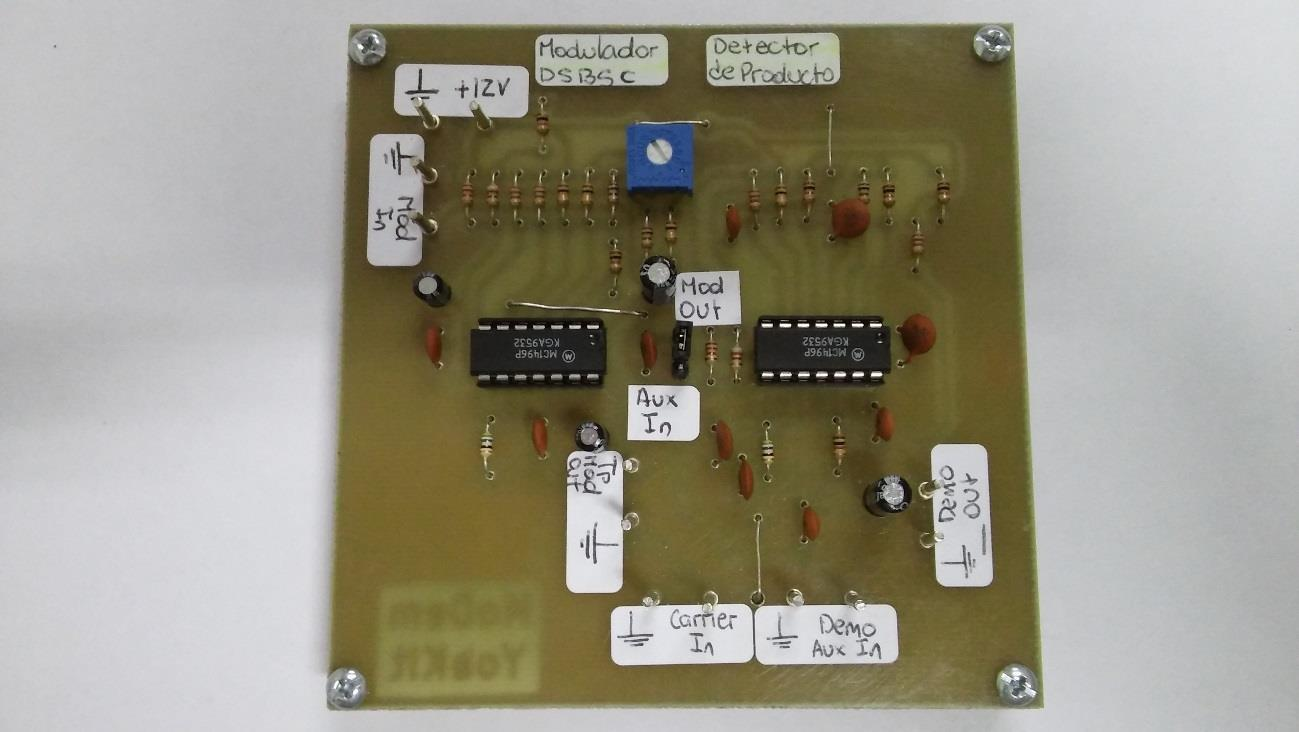
\includegraphics[width=0.555\textwidth]{pictures/kit_dsbsc.png}
    \caption{Placa de laboratorio del Kit N° 5.}
    \label{fig.dsbsc:kit}
\end{figure}

Con el módulo energizado, procedimos a inyectar las señales provenientes de ambos generadores de funciones en los
terminales de entrada correspondientes:
\begin{itemize}
    \item Canal 1 (amarillo, conector Mod In): señal modulante senoidal con frecuencia $f_m \approx 10\kHz$
          y nivel nominal de $30\mVrms$.
    \item Canal 2 (cian, conector Carrier In): señal portadora senoidal con frecuencia $f_c \approx 100\kHz$
          y nivel nominal de $60\mVrms$.
\end{itemize}

En la figura \ref{fig.dsbsc:entradas} se observa la captura de ambas señales efectuada en el osciloscopio digital.
Los valores medidos por el instrumental fueron $V_{\mathrm{rms}}(1) = 30{,}2\mV$, con una frecuencia
$f_1 = 10{,}25\kHz$, y $V_{\mathrm{rms}}(2) = 61{,}9\mV$ para la portadora, verificando el ajuste riguroso
de las consignas de polarización recomendadas en la hoja de datos del MC1496.

\begin{figure}[!ht]
    \centering
    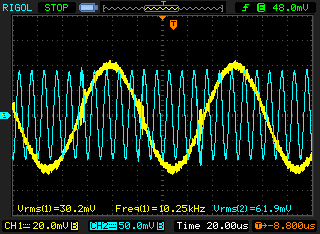
\includegraphics[width=0.68\textwidth]{images/NewFile0.png}
    \caption{Señales de entrada al modulador.}
    \label{fig.dsbsc:entradas}
\end{figure}

\section{Respuesta Temporal del Modulador DSB-SC}
Conectamos el Canal 1 del osciloscopio al terminal de salida del modulador (conector Mod Out) manteniendo
la portadora en el Canal 2 para referencia de fase. La señal obtenida se ilustra en la figura \ref{fig.dsbsc:modulada}.
El osciloscopio registró una tensión eficaz de $V_{\mathrm{rms}}(1) = 207\mV$ y una frecuencia de conmutación de
$100{,}0\kHz$.

\begin{figure}[!ht]
    \centering
    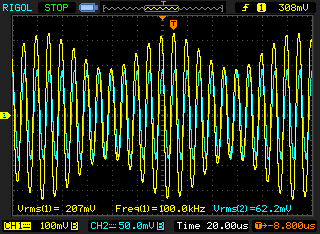
\includegraphics[width=0.68\textwidth]{images/NewFile1.png}
    \caption{Señal modulada en DSB-SC comparada con la portadora de referencia.}
    \label{fig.dsbsc:modulada}
\end{figure}

Al examinar la forma de onda temporal de la figura \ref{fig.dsbsc:modulada}, se destaca una característica distintiva
de la modulación DSB-SC: la envolvente se anula periódicamente en coincidencia con los cruces por cero de la señal
modulante. En dicho instante, la fase de la portadora interna experimenta un salto abrupto de $180^\circ$ ($\pi\unit{\radian}$),
fenómeno predicho teóricamente por el cambio de signo de la función modulante $e_m(t)$. A diferencia de la modulación
AM convencional, la envolvente no describe la forma de la señal de información, sino su valor absoluto rectificado.

\section{Influencia de la Amplitud de la Señal Modulante}
A continuación, variamos progresivamente la amplitud de la señal en banda base inyectada en Mod In para evaluar
el comportamiento temporal y espectral de la celda de multiplicación. Las capturas temporales registradas para
tres niveles crecientes de excitación se presentan en la figura \ref{fig.dsbsc:amplitud_var}.

\begin{figure}[!ht]
    \centering
    \begin{subfigure}[t]{0.32\textwidth}
        \centering
        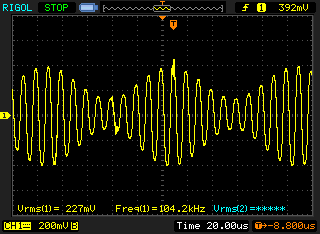
\includegraphics[width=\textwidth]{images/NewFile2.png}
        \caption{Nivel bajo.}
        \label{fig.dsbsc:amp1}
    \end{subfigure}\hfill
    \begin{subfigure}[t]{0.32\textwidth}
        \centering
        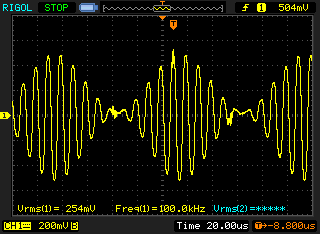
\includegraphics[width=\textwidth]{images/NewFile3.png}
        \caption{Nivel intermedio.}
        \label{fig.dsbsc:amp2}
    \end{subfigure}\hfill
    \begin{subfigure}[t]{0.32\textwidth}
        \centering
        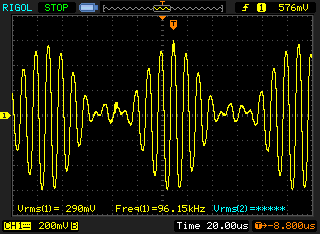
\includegraphics[width=\textwidth]{images/NewFile4.png}
        \caption{Nivel elevado.}
        \label{fig.dsbsc:amp3}
    \end{subfigure}
    \caption{Evolución temporal de la señal DSB-SC ante incrementos en la amplitud de la banda base.}
    \label{fig.dsbsc:amplitud_var}
\end{figure}

En DSB-SC no existe el concepto de sobremodulación por cruce de portadora debido a la ausencia intrínseca de esta
última.

\begin{figure}[!ht]
    \centering
    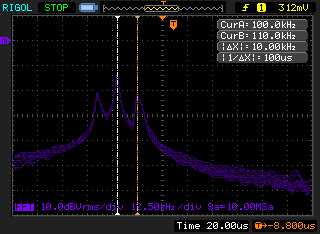
\includegraphics[width=0.68\textwidth]{images/NewFile5.png}
    \caption{Espectro en frecuencia (FFT) de la señal DSB-SC para $f_m = 10\kHz$.}
    \label{fig.dsbsc:fft_10k}
\end{figure}

En la figura \ref{fig.dsbsc:fft_10k} se presenta el análisis espectral obtenido mediante la función FFT del osciloscopio
para el caso nominal. Los cursores del instrumento muestran:
\begin{itemize}
    \item Cursor A: fijado en la frecuencia de la portadora, $100{,}0\kHz$.
    \item Cursor B: ubicado en el pico de la banda lateral superior, $110{,}0\kHz$.
    \item Intervalo entre cursores: $|\Delta X| = 10{,}00\kHz$, coherente con la frecuencia modulante inyectada.
\end{itemize}
Se observa con claridad la generación de los dos lóbulos laterales en $90\kHz$ y $110\kHz$. \textbf{NOTA:} En teoría, el pico de la
portadora, no debería aparecer en el espectro de frecuencia. Así y todo, lo hace, por lo que suponemos que el kit está
mal etiquetado, o bien está fallando. El espectro obtenido es el caracteristico de una modulacion AM o doble banda
lateral con portadora.

\section{Influencia de la Frecuencia Modulante}
Para analizar la dependencia espectral y temporal respecto a la frecuencia de banda base, modificamos la señal
modulante manteniendo fija la portadora en $100\kHz$. Evaluamos tres condiciones de ensayo: $f_m = 10\kHz$, $f_m =
1\kHz$ y $f_m = 20\kHz$

\begin{figure}[!ht]
    \centering
    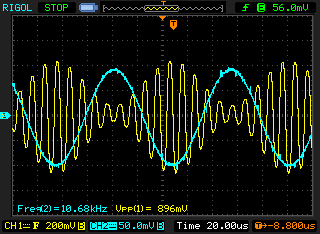
\includegraphics[width=0.45\textwidth]{images/NewFile6.png}
    \caption{Señal modulada (CH1) y modulante (CH2).}
    \label{fig.dsbsc:freq_10k}
\end{figure}

\begin{figure}[!ht]
    \centering
    \begin{subfigure}[t]{0.45\textwidth}
        \centering
        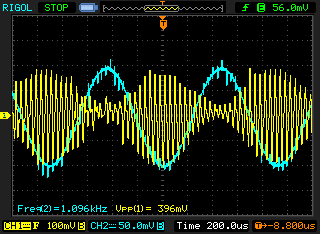
\includegraphics[width=\textwidth]{images/NewFile8.png}
        \caption{Dominio del tiempo.}
        \label{fig.dsbsc:freq_1k_time}
    \end{subfigure}\hfill
    \begin{subfigure}[t]{0.45\textwidth}
        \centering
        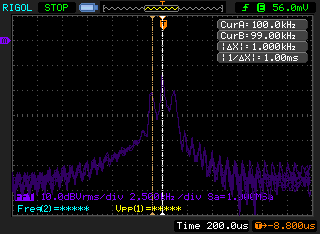
\includegraphics[width=\textwidth]{images/NewFile9.png}
        \caption{Dominio en frecuencia.}
        \label{fig.dsbsc:freq_1k_fft}
    \end{subfigure}
    \caption{Respuesta de modulación DSB-SC para $f_m \approx 1\kHz$.}
    \label{fig.dsbsc:freq_1k}
\end{figure}

\begin{figure}[!ht]
    \centering
    \begin{subfigure}[t]{0.45\textwidth}
        \centering
        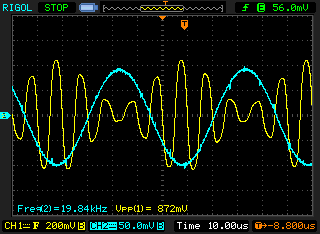
\includegraphics[width=\textwidth]{images/NewFile7.png}
        \caption{Dominio del tiempo.}
        \label{fig.dsbsc:freq_20k_time}
    \end{subfigure}\hfill
    \begin{subfigure}[t]{0.45\textwidth}
        \centering
        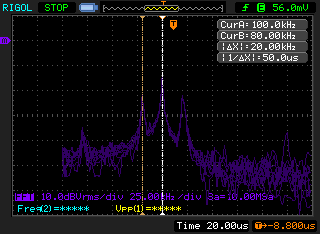
\includegraphics[width=\textwidth]{images/NewFile10.png}
        \caption{Dominio en frecuencia.}
        \label{fig.dsbsc:freq_20k_fft}
    \end{subfigure}
    \caption{Respuesta de modulación DSB-SC para $f_m \approx 20\kHz$.}
    \label{fig.dsbsc:freq_20k}
\end{figure}

\section{Demodulación Sincrónica}
La recuperación de la señal de información a partir de una onda DSB-SC no puede implementarse mediante detectores de
envolvente convencionales (rectificadores con diodo), ya que la envolvente rectificada presentaría distorsión severa
por los saltos de fase de $180^\circ$. Se requiere obligatoriamente una detección coherente o sincrónica.

El receptor multiplica la señal recibida $v_{\mathrm{DSB}}(t)$ por una portadora local reinyectada $v_{\mathrm{c,loc}}(t) = \cos(\omega_c t)$:
\begin{gather*}
    v_{\mathrm{det}}(t) = v_{\mathrm{DSB}}(t) \cos(\omega_c t) = \left[e_m(t) \cos(\omega_c t)\right] \cos(\omega_c t) = e_m(t) \cos^2(\omega_c t) \\
    v_{\mathrm{det}}(t) = \frac{1}{2} e_m(t) + \frac{1}{2} e_m(t) \cos(2\omega_c t) \nonumber
\end{gather*}
Sustituyendo el tono modulante $e_m(t) = E_m \cos(\omega_m t)$:
\begin{equation}
    v_{\mathrm{det}}(t) = \frac{E_m}{2} \cos(\omega_m t) + \frac{E_m}{4} \cos\left((2\omega_c + \omega_m)t\right) + \frac{E_m}{4} \cos\left((2\omega_c - \omega_m)t\right)
    \label{eq.dsbsc:deteccion}
\end{equation}
La ecuación (\ref{eq.dsbsc:deteccion}) demuestra la aparición de la señal en banda base de baja frecuencia
($\omega_m$) junto con productos centrados en el doble de la frecuencia portadora ($2\omega_c \approx 200\kHz$).
Mediante un filtro paso bajo, estas componentes de radiofrecuencia se eliminan por completo.

Conectamos la punta de prueba en la salida Demo Out del kit. En la figura \ref{fig.dsbsc:demodulacion} se observa la señal
recuperada en el Canal 1 ($500\mV/\text{div}$). La forma de onda reproduce fielmente el tono senoidal
original de $10\kHz$ de la banda base, mientras que en el Canal 2 se aprecia el remanente de alta frecuencia del proceso
de conmutación antes de su rechazo final.

\begin{figure}[!ht]
    \centering
    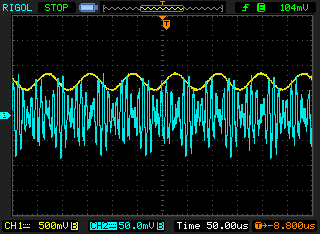
\includegraphics[width=0.68\textwidth]{images/NewFile11.png}
    \caption{Señal recuperada en la salida tras la demodulación.}
    \label{fig.dsbsc:demodulacion}
\end{figure}

\section{Cuantificación del Rechazo de Portadora}
Desconectando la señal modulante de entrada ($e_m(t) = 0$)  y manteniendo aplicada la portadora de $100\kHz$ y
$60\mVrms$, la salida del modulador debería ser nula. Sin embargo, debido a las asimetrías
térmicas y a la dispersión en las características de los transistores integrados, se genera una fuga de portadora no
deseada en el terminal de salida.

El kit dispone de un preset de ajuste que modifica la polarización diferencial de corriente en los emisores del par
multiplicador. Procedimos a medir la tensión de portadora residual en los dos extremos operativos del ajuste:
\begin{itemize}
    \item Nivel máximo de portadora no deseada (desbalance forzado): $V_{\mathrm{max}} = 600\mV$.
    \item Nivel mínimo de portadora residual alcanzado tras calibración cuidadosa del preset: $V_{\mathrm{min}} \approx 127\mV$.
\end{itemize}
La capacidad de supresión de portadora del modulador balanceado se calcula mediante la relación logarítmica:
\begin{equation}
    \text{Atenuación}_{\mathrm{portadora}} = 20 \log_{10}\left(\frac{V_{\mathrm{max}}}{V_{\mathrm{min}}}\right) = 20 \log_{10}\left(\frac{600\mV}{127{,}4\mV}\right) \approx 13{,}46\dB
    \label{eq.dsbsc:rechazo_calculo}
\end{equation}
Este valor de $13{,}46\dB$ corrobora experimentalmente que el preset de balance permite mitigar sustancialmente la fuga
de portadora directa, optimizando el rendimiento espectral del sistema DSB-SC.
